\chapter{Математические модели основанные на ОДУ}

\textbf{Дифференциальное уравнение} -- это уравнение, в которое входят
производные функции, которые надо найти. Порядок $du$ определяется
наивысшим порядком производной. ДУ называется \textbf{обыкновенным},
если функция зависит только от одного переменного.

\section{Сведение дифференциального уравнения $n$-го порядка к системе
дифференциальных уравнений 1-го порядка}

\begin{equation*}
    \begin{matrix}
        u^{(n)} = f (x, u, u', u'', ..., u^{(n-1)}) \\
        \\
        u' = u_1 \\
        \\
        u'' = u_2 \\
        \\
        u'_k = (u^{(k)})' = u^{(k+1)} = u_{k+1}
    \end{matrix}
\end{equation*}

\begin{equation*}
    \begin{cases}
        u'=u_1 \\
        u_1'=u_2 \\
        \vdots \\
        u'_{n-1} = f(x, u, u_1, u_2 .. u_{n-1}) \\
    \end{cases}
\end{equation*}

Система уравнений первого порядка выглядит следующим образом

\begin{equation*}
    u'_k(x) = f_k(x, u_1, u_2, ..., u_n),
    k = \overline{1,n}
\end{equation*}

Уравнение $n$-го порядка содержит $n$ производных
констант. Решение с этими константами определяет общее решение.
Для выделение частного решения, константы должны быть определены,
для этого ставятся дополнительные условия. Если все условия ставятся
в одной точке, то это называется \textbf{задача Коши}. Если все условия
заданы в разных точках, то называется \textbf{краевая задача}.

\section{Задача Коши для ОДУ}

\subsection{Методы решения}

\begin{enumerate}
    \item \textbf{Точный метод} --
        в ряде случаев представляет из себя неявную функцию, тогда
        для получения зависимости $u(x)$ необходимо применять
        численные методы (например, поовинного деления).
    \item \textbf{Приближенный математический метод} --
        например, метод Пикара.
    \item \textbf{Численный метод} --
        универсальный, подходит для тех, у кого нет аналитического
        решения и для тех, у кого его нет. Получаем только
        частные решения.
\end{enumerate}

\subsection{Численные методы решения}

\subsubsection{Предварительные замечания}

Рассматриваем уравнение первого порядка

\begin{equation*}
    \begin{cases}
        u'(x) = f(x, u(x)) \\
        u(\xi) = \eta \\
        a \le x \le b \\
    \end{cases}
\end{equation*}

В области интегрирования от $a$ до $b$ вводится сетка

\begin{figure}[H]
    \centering
    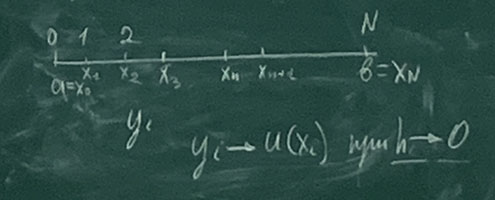
\includegraphics[scale=0.8]{img/grid.jpg}
\end{figure}

\begin{equation*}
    \omega = \{
        x_i : a = x_0 < x_1 < x_2 < ... < x_n < x_{n+1} < ... < x_N
    \}
\end{equation*}

\begin{equation*}
    \begin{matrix}
        x_n - x_{n-1} = h_n - \text{ шаг} \\
        h_n = \text{const} \\
        w_h = \{ x_i : x_i = a + i \cdot h, i = \overline{0,N} \} \\
    \end{matrix}
\end{equation*}

Функция, полученная на выбранной сетке в результате применения
численного метода называется \textbf{сеточная функция}

\subsubsection{Понятие сходимости}

Фиксируется некий $x$.

\begin{equation*}
    \begin{matrix}
        x_{ij}, h \to 0, i \to \infty \\
        x_i = a + ih \\
        |y_i - u(x_i)| \to 0, h \to 0 \\
        |y_i - u(x_i)| = O(h^p), h \to 0
    \end{matrix}
\end{equation*}

Сеточная функция имеет $p$-й порядок точности, если абсолютная
величина разности -- шаг в степери $p$.

\subsubsection{Как найти решение численным методом}

Разложим ряд Тейлора

\begin{equation*}
    u_{n+1} = u_n + \frac{h}{1!} u'_n + \frac{h^2}{2!} u_n'' +
    \frac{h^3}{3!} u_n''' + ...
\end{equation*}

\begin{equation*}
    u'_n = f(x_n, u_n) \\
\end{equation*}

\begin{equation*}
    u''_n = (u_n') = \frac{df}{dx} (x, u) \bigg|_{x=x_n} =
    f'_x (x_n, u_n) + f'_uf \bigg|_{x=x_n}
\end{equation*}

\begin{equation*}
    y_{n+1} = y_n + hf(x_n, u_n) - \text{ метод Эйлера}
\end{equation*}

Получим формулы второго порядка точности методом Рунге-Кутта.

\begin{equation}\label{eq:y1}
    y_{n+1} = y_n + h_n f(x_n,y_n) + \frac{h_n^2}{2!} u_n''
\end{equation}

\begin{equation*}
    u_m'' = (u_n)' = \frac{df(x,u)}{dx} \bigg|_{x_n} = f'_x(x_n, y_n) +
    f'_y(x_n, y_n) \cdot f(x_n, y_n)
\end{equation*}

\begin{equation}\label{eq:y2}
    y_{n+1} = y_n + h_n \cdot f(x_n, y_n) + \frac{h_n^2}{2}
    \bigg[ f_x'(x_n, y_n) + f_y'(x_n, y_n) \cdot f(x_n, y_n) \bigg]
\end{equation}

\begin{equation*}
    u_n'' = \frac{df}{dx} =
    \frac{f(x_n + \gamma h_n, y_n d \delta h_n) - f(x_n, y_n)}{\Delta x}
\end{equation*}

Подставим в \ref{eq:y1}

\begin{equation*}
    y_{n+1} = y_n + h_n f(x_n, y_n) + \frac{h_n^2}{2!}
    \bigg[
    \frac{f(x_n + \gamma h_n, y_n + \delta h_n) - f(x_n, y_n)}{\Delta x}
    \bigg] =
\end{equation*}

\begin{equation}\label{eq:y3}
    = y_n + h_n \bigg[ \beta f(x_n, y_n) + \alpha f(x_n + \gamma h_n, y_n + \delta h_n) \bigg]
\end{equation}

\begin{equation*}
    y_{n+1} = y_n + h_n \bigg\{ \beta f(x_n, y_n + \alpha \big[
    f(x_n, y_n) + f_x' \gamma h_n + f_y' \delta h_n \big] \bigg\}
\end{equation*}

\begin{equation}\label{eq:y4}
    = y_n + h_n (\alpha + \beta) f(x_n, y_n) + \alpha \gamma h_n^2 f'_x
    + \alpha \delta y h_n^2
\end{equation}

Сравним \ref{eq:y4} и \ref{eq:y2}. Видим

\begin{equation*}
    \begin{cases}
        \alpha + \beta = 1 \\
        \alpha \gamma = \frac{1}{2} \\
        \alpha \delta = \frac{1}{2} f(x_n, y_n) \\
    \end{cases}
\end{equation*}

\begin{equation*}
    \begin{cases}
        \beta = 1 - \alpha \\
        \gamma = \frac{1}{2\alpha} \\
        \delta = \frac{1}{2\alpha} f(x_n, y_n) \\
    \end{cases}
\end{equation*}

Кончательно подставляя найденные параметры в \ref{eq:y4} получим
рассчетную формулу.

\begin{equation}
    y_{n+1} = y_n + h_n
    \bigg[ (1-\alpha) f(x_n, y_n) + \alpha f \big( x_n + \frac{h_n}{2},
    y_n + \frac{h_n}{2} f(x_n, y_n) \big) \bigg]
\end{equation}

Семейство однопараметрических формул Рунге-Кутта второго порядка

Обычно на практике $\alpha = 1$ или $\frac{1}{2}$, $O(\max h_n^2)$,
$O(h^2)$

\underline{$\alpha = 1$}

\begin{equation*}
    y_{n+1} = y_n + h_n
    f\big(x_n + \frac{h_n}{2}, y_n + \frac{h_n}{2} f(x_n, y_n)\big)
\end{equation*}

\begin{enumerate}
    \item $y_{n + \frac{1}{2}} = y_n + \frac{h_n}{2}f(x_n, y_n)$
    \item $y'_{n+\frac{1}{2}} = f(x_{n + \frac{1}{2}}, y_{n + \frac{1}{2}})$
    \item $y_{n+1} = y_n + h_n \cdot y'_{n + \frac{1}{2}}$
\end{enumerate}

\subsection{Метод Рунге-Кутта четвертого порядка точности}

\begin{equation*}
    y_{n+1} = y_n + \frac{k_1 + 2k_2 + 2k_3 + k_4}{6}
\end{equation*}

\begin{equation*}
    k_1 = h_n f(x_n, y_n)
\end{equation*}

\begin{equation*}
    k_2  =h_n f(x_n + \frac{h_2}{2}, y_n + \frac{k_1}{2})
\end{equation*}

\begin{equation*}
    k_3 = h_n f(x_n + \frac{h_n}{2}, y_n + \frac{k_2}{2})
\end{equation*}

\begin{equation*}
    k_4 = h_n f(x_n + h_n, y_n + k_3)
\end{equation*}

\subsubsection{Обощение формулы на случай двух переменных}

\begin{equation*}
    \begin{cases}
        u'(x) = f(x,u,v) + y \\
        v'(x) = u(x,u,v) + z \\
        v(\xi) = v_0 \\
        u(\xi) = u_0 \\
    \end{cases}
\end{equation*}

\begin{equation*}
    y_{n+1} = y_n + \frac{k_1 + 2k_2 + 2k_3 + k_4}{6},
\end{equation*}

\begin{equation*}
    z_{n+1} = z_n + \frac{q_1 + 2q_2 + 2q_3 + q_4}{6}
\end{equation*}

где

\begin{equation*}
    k_1 = h_n f(x_n, y_n, z_n), q_1 = h_n \varphi (x_n, y_n, z_n)
\end{equation*}

\begin{equation*}
    k_2 = h_n f (x_n + \frac{h_n}{2}, y_n + \frac{k_1}{2}, z_n + \frac{q_1}{2}), q_2 = h_n \varphi(x_n + \frac{h_n}{2}, y_n + \frac{k_1}{2}, z_n + \frac{q_1}{2})
\end{equation*}

\begin{equation*}
    k_3 = h_n f (x_n + \frac{h_n}{2}, y_n + \frac{k_2}{2}, z_n + \frac{q_2}{2}), q_3 = h_n \varphi(x_n + \frac{h_n}{2}, y_n + \frac{k_2}{2}, z_n + \frac{q_2}{2})
\end{equation*}

\begin{equation*}
    k_4 = h_n f (x_n + h_n, y_n + k_3, z_n + q_3, q_4 = h_n \varphi(x_n + h_n, y_n + k_3, z_n + q_3)
\end{equation*}

\subsection{Приемущества метода Рунге-Кутта}

\begin{itemize}
    \item Они явные. Для перехода из $n$ в $n+1$ узел надо строго
        фиксированное количество операций
    \item Формулы достаточно точные
    \item Формулы позволяют вести подсчеты с переменным шагом
\end{itemize}

\subsection{Лабораторная работа 2}

\textbf{Тема}: ОДУ. Задача Коши для системы из двух уравнений

Имеется разрядный контур ($R_\text{к}, C_\text{к}, L_\text{к}$)

Начальный заряд конденсатора $U_{0 \text{к}}$

\begin{equation*}
    R_p(I) = \frac{l_{\text{э}}}{2 \pi R^2 \int_0^1 \sigma(T(z))zdz}
\end{equation*}

\begin{figure}[H]
    \centering
    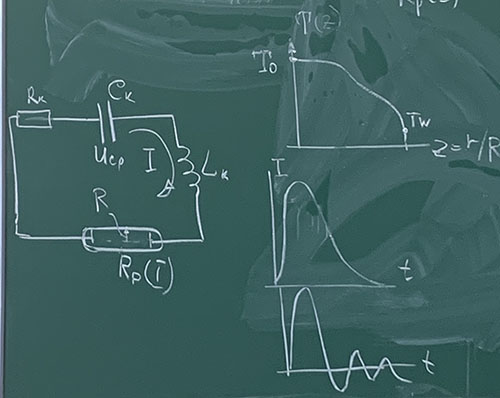
\includegraphics[scale=0.7]{img/lab_02.jpg}
\end{figure}

Система уравнений

\begin{equation*}
    \begin{cases}
        L_\text{к}\frac{dI}{dt} + (R_\text{к} + R_p) I - U_c = 0 \\
        C_\text{к} \frac{dU_c}{dt} = -I \\
    \end{cases}
\end{equation*}

\begin{equation*}
    t = 0, I = I_0, U_c = U_{c0}
\end{equation*}

\begin{equation*}
    \begin{cases}
        \frac{dI}{dt} = \frac{1}{L_\text{к}} (U_c...) \\
        \frac{dU_c}{dt} = -\frac{T}{C_\text{к}} \\
    \end{cases}
\end{equation*}

\subsubsection{Метод решения Рунге-Кутт 2-го порядка}

\begin{equation*}
    y_{n+1} = y_n + h_n \bigg[ (1-\alpha) f(x_n, y_n) +
        \alpha f(x_n + \frac{h_n}{2\alpha},
    y_n + \frac{h_n}{2\alpha} f(x_n, y_n) \bigg],
    \alpha = 1 or \frac{1}{2}
\end{equation*}

\subsubsection{Метод решения Рунге-Кутт 4-го порядка}

\begin{equation*}
    y_{n+1} = y_n + \frac{k_1 + 2k_2+2k_3+k_4}{6},
    z_{n+1} = z_n + \frac{q_1 + 2q_2 + 2q_3 + q_4}{6}
\end{equation*}

\begin{equation*}
    k_i, q_i, i = \overline{1;4} - \text{известные}
\end{equation*}

\subsubsection{Входные данные}

\begin{table}[H]
    $T_w = 2000K$

    \centering
    \begin{tabular}{c|c|c}
        $I$, А & $T_0$, К & m \\
        \hline
        0.5 & 6400 & 0.4 \\
            & & \\
            & & \\
    \end{tabular}
\end{table}

\begin{table}[H]
    \centering
    \begin{tabular}{c|c}
        $T$, К & $\sigma, \frac{1}{\text{О} \cdot \text{см}}$ \\
        \hline
        4000 & 0.031 \\
             & \\
             & \\
    \end{tabular}
\end{table}

\begin{equation*}
    \begin{matrix}
        R = \\
        L_\text{э} = \\
        L_\text{к} = 187 \cdot 10^{-6} \text{Гн} \\
        R_\text{к} = 0.25 \text{Ом} \\
        U_{c0} = \\
        I_0 = 0.5 ... 3 \text{А} \\
        \tau - \text{Шаг} \sim 1 \cdot 10^{-6} \text{с} \\
        t_p - \text{Полное время импульса}
    \end{matrix}
\end{equation*}

В интерфейс: $L_\text{к}, R_\text{к}, U_{c0}, I_0, \tau, t_p$

\subsubsection{Выходные данные}

\begin{figure}[H]
    \centering
    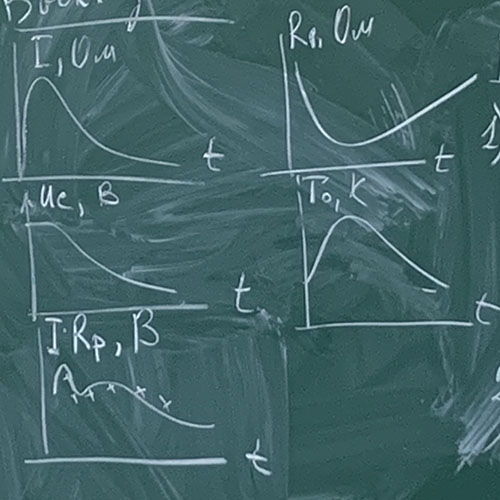
\includegraphics[scale=0.7]{img/lab_02_input.jpg}
\end{figure}

\subsubsection{Общий вид задачи}

\begin{equation*}
    \begin{cases}
        u'(t) = f(t,u,v) \\
        v'(t) = \varphi (t,u,v) \\
    \end{cases}
\end{equation*}

\subsection{Оценим погешность методов}

\subsubsection{Методы второго порядка}

\begin{equation*}
    u'(x) = f(x)
\end{equation*}

\begin{equation*}
    \int_{x_n}^{x_{n+1}} \frac{fu}{dx} dx =
    \int_{x_n}^{x_{n+1}} f(x) dx
\end{equation*}

\begin{equation*}
    u_{n+1} = u_n + \int_{x_n}^{x_{n+1}} f(x) dx
\end{equation*}

\paragraph{$\alpha = 1$}

\begin{equation*}
    y_{n+1} = y_n + h f(x_n + \frac{h}{2})
\end{equation*}

\begin{equation*}
    R = \frac{x_N - x_0}{24} \cdot h^2
    \underset{x_0 \le x \le x_N}{\max} |f''(x)|
\end{equation*}

\paragraph{$\alpha = \frac{1}{2}$}

\begin{equation*}
    y_{n+1} = y_n + \frac{h}{2} \bigg[ f(x_n) + f(x_n + h) \bigg]
\end{equation*}

\begin{equation*}
    R = \frac{x_N - x_0}{12} \cdot h^2
    \underset{x_0 \le x \le x_N}{\max} |f''(x)|
\end{equation*}

\subsubsection{Методы четвертого порядка}

\begin{equation*}
    u'(x) = f(x)
\end{equation*}

\begin{equation*}
    y_{n+1} = y_n + \frac{h}{6} \bigg[ f(x_n) +
    4 f(x_n + \frac{h}{2} + f(x_n + h) \bigg]
\end{equation*}

\begin{equation*}
    R = \frac{x_N - x_0}{180} \bigg( \frac{h}{2} \bigg) ^4
    \underset{x_0 \le x \le x_N}{\max} |f^{IV}(x)| =
    \frac{x_N - x_0}{2880} h^4
    \underset{x_0 \le x \le x_N}{\max} |f^{IV}(x)|
\end{equation*}

\subsection{Многошаговые методы (метод Адамса)}

Для перехода из $x_n$ в $x_{n+1}$ используются предыдущие
шаги $\{x_{n-1}, x_{n-2}, x_{n-3} ...\}$

В качестве примера рассмотрим \textbf{метод Адамса}

К некоторому моменту известно $y_n, y_{n-1}, y_{n-2}, y_{n-3}$
(применен метод Рунге-Кутта)

\begin{equation*}
    u'(x) = f(x, \underbrace{u(x)}_\text{интегральная кривая})
    \equiv F(x)
\end{equation*}

\begin{multline*}
    F(x) = F(x_n) + (x - x_n) F(x_n, x_{n-1}) +
    (x-x_n)(x - x_{n-1}) F(x_n, x_{n-1}, x_{n-2}) + \\
    + (x - x_n) (x - x_{n-1}) (x - x_{n-2}) F(x_n, x_{n-1}, x_{n-2},
    x_{n-3})
\end{multline*}

Например,

\begin{equation*}
    F(x_n, x_{n-1}) = \frac{F(x_n) - F(x_{n-1})}{x_n - x_{n-1}} =
    \frac{f(x_n, y_n) - f(x_{n-1}, y_{n-1})}{x_n - x_{n-1}}
\end{equation*}

Интегральная форма дифференциального уравнения

\begin{equation*}
    u_{n+1} = u_n + \int_{x_n}^{x_{n+1}} f(x, u(x)) dx =
    u_n + \int_{x_n}^{x_{n+2}} F(x) dx
\end{equation*}

Подставляя $F(x)$, представленного полиномом Ньютона, получим

\begin{multline*}
    y_{n+1} = y_n + h_n F(x_n) +
    \frac{1}{2} h_n^2 F(x_n, x_{n+1}) +
    \frac{1}{6} h_n^2 (2h_n + 3 h_{n-1})
    F(x_n, x_{n-1}, x_{n-2}) + \\
    + \frac{1}{12} h_n^2 (3h_n^2 + 8h_nh_{n-1} + 4h_nh_{n-2} +
    6h_{n-1}^2 + 6 h_{n-1}h_{n-2}) F(x_n, x_{n-1}, x_{n-2}, x_{n-3})
\end{multline*}

где $h_n = x_{n+1} - x_n$, $h_{n-2} = x_{n-1}-x_{n-2}$

Это формула Адамса, у нее четвертый порядок точности.
Если $h_n = \text{const} = h$, формула упрощается.
Порядок погрешности при постоянном шаге:

\begin{equation*}
    R \sim \frac{251}{750} h^4 \sim \frac{h^4}{3}
\end{equation*}

Преимущество метода Адамса в том, что для перехода в следующий
узел правая часть вычисляется один раз. В то время, как в методе
Рунге-Кутта того же порядка точности правую часть надо вычислять
4 раза. Это преимущество нивелируется, тем, что точность метода
Адамса ниже. Оценка погрешности показывает, что последняя в 960
раз больше в методе Адамса, чем в методе Рунге-Кутта, поэтому
шаг в методе Рунге-Кутта может быть в 5 - 5.5 раз больше.
Начальный участок, необходимо посчитать другим методом
(то есть надо менять метод).

\subsection{Оценка погрешности расчета с
использованием формулы Рунге-Кутта}

Расчет проводится на двух сетках с отличающимся шагом
$h, mh$. Расчет можно провести на узлах, которые совпадают.
Проведя расчеты в двух сетках, можно оценить абсолютную
погрешность:

\begin{equation*}
    \Delta y = \frac{y(x, h) - y(x, mh)}{m^p - 1}
\end{equation*}

где $p$ -- порядок метода, $m$ -- различие сетки

\begin{itemize}
    \item $p=1$ -- метод Эйлера
    \item $p=2$ -- метод Рунге-Кутта
    \item $p=4$ -- метод Рунге-Кутта
    \item $p=4$ -- метод Адамса
\end{itemize}

$m > 1$ -- разряжение сетки, $m < 1$ -- сгущение сетки

Сгущая или разряжая сетку и применяя формулу Рунге-Кутта можно
оценить погрешность.

\subsection{Неявные методы}

\subsubsection{Метод Эйлера}

\begin{equation*}
    y_{n+1} = y_n + hf(x_{n+1}, y_{n+1})\ \ \ + O(h)
\end{equation*}

\subsubsection{Метод Трапеций}

\begin{equation*}
    u_{n+1} = u_n + \int_{x_n}^{x_{n+1}} f(x, u(x)) dx
\end{equation*}

\begin{equation*}
    y_{n+1} = y_n + \frac{h}{2} \bigg[ f(x_n, y_n) +
    f(x_{n+1}, y_{n+1}) \bigg]\ \ \ \ \ + O(h)
\end{equation*}

\subsubsection{Методы Гира}

\begin{equation*}
    \frac{3}{2} y_{n+1} - 2y_n + \frac{1}{2} y_{n-1} =
    hf(x_{n+1}, y_{n+1}) \ \ \ \ \ + O(h^2)
\end{equation*}

\begin{equation*}
    \frac{11}{6} y_{n+1} - 3y_n + \frac{3}{2} y_{n-1} - \frac{1}{3}
    y_{n-2} = hf(x_{n+1}, y_{n+1}) \ \ \ \ \ +O(h^3)
\end{equation*}

\subsubsection{Метод последовательных приближений}

\begin{equation*}
    \varphi(y) = 0
\end{equation*}

\begin{equation*}
    y_{n+1}^{(1+1)} = \Psi (y_{n+1}^{(1)})
\end{equation*}

\begin{equation*}
    y^{(0)} = y_n, |\Psi'| < 1
\end{equation*}

\section{ОДУ. Краевые задачи}

\subsection{Постановка в общем виде}

\begin{equation*}
    u_k'(x) = f_k (x, u_1, u_2, ..., u_n)
\end{equation*}

\begin{equation*}
    \varphi_k(u_1(\xi_k), u_2(\xi_k),...,u_n(\xi_k), k = \overline{1;n}
\end{equation*}

\subsection{Классификация методов}

\begin{itemize}
    \item Аналитические
    \item Приближенно-аналитические

        \begin{itemize}
            \item Коллокаций
            \item Галеркина
            \item Наименших квадратов
        \end{itemize}

    \item Численные

        \begin{itemize}
            \item Разностные
            \item Проекционно-сеточные
        \end{itemize}
\end{itemize}

\subsection{Разностный метод. Существование, единственность, сходимость
разностного решения к точному}

\begin{equation*}
    u''(x) - p(x)u(x) = f(x)
\end{equation*}

$p(x), f(x)$ -- заданные функции. Пусть $p(x) > 0$

\begin{equation*}
    u(a) = \alpha
\end{equation*}

\begin{equation*}
    u(b) = \beta
\end{equation*}

\begin{equation*}
    a \le x \le b
\end{equation*}

\begin{equation*}
    \omega_n = \{ x_n : x_n = a + nh, n = \overline{0, N} \}
\end{equation*}

Получим простейшую разностную схему методом разнстной апроксимации.

\begin{equation*}
    u''_n = \frac{u_{n-1} - 2 u_n + u_{n+1}}{h^2} - \frac{1}{12} h^2
    u^{IV} (\xi)
\end{equation*}

\begin{equation*}
    x_{n-1} \le \xi \le x_{n+1}
\end{equation*}

\begin{equation*}
    \frac{y_{n-1} - 2 y_n + y_{n+1}}{h^2} - p_ny_n = f_n,
\end{equation*}

\begin{equation*}
    p_n = p(x_n), f_n = f(x_n)
\end{equation*}

\begin{equation*}
    \begin{matrix}
        y_0 = \alpha \\
        y_N = \rho \\
    \end{matrix}
\end{equation*}

\begin{equation*}
    n = \overline{1, N-1}
\end{equation*}

\begin{equation}\label{eq:diagonalmatrix}
    y_{n-1} - (2 + h^2 p_n) y_n + y_{n+1} = h^2 f_n
\end{equation}

\begin{equation*}
    z_n = y_n - u_n
\end{equation*}

Покажем, что выписанная разностная схема имеет второй порядок точности.
То есть погрешность сеточной функции стремится к нулю

\begin{equation*}
    O(h^2) \text{ при } h \to 0
\end{equation*}

Получим

\begin{equation*}
    \frac{u_{n-1} - 2u_n + u_{n+1}}{h^2} - \frac{1}{12} h^2 u^{IV} (\xi) -
    p_nu_n = f_n
\end{equation*}

\begin{equation}\label{eq:un-1}
    u_{n-1} - (2 + h^2p_n) u_n + u_{n+1} = \frac{1}{12} h^4 u^{IV}(\xi) +
    f_nh^2
\end{equation}

Из \ref{eq:diagonalmatrix} вычтем \ref{eq:un-1}

\begin{equation*}
    z_{n-1} - (2+h^2p_n)z_n + z_{n+1} = -\frac{1}{12} h^4 u^{IV}(\xi)
\end{equation*}

\begin{equation*}
    \big|(2+h^2p_n)z_n\big| = \big|z_{n-1} + z_{n+1} + \frac{1}{12} h^4 u^{IV}(\xi)\big|
\end{equation*}

\begin{equation*}
    \big|(2+h^2p_n)z_n\big| \le \big|z_{n-1}\big| + \big|z_{n+1}\big| + \frac{h^4}{12}
    \big|u^{IV}(\xi)\big|
\end{equation*}

\begin{equation*}
    \big| (2+h^2p_n)z_m \big| \le 2 \big| z_m \big| + \frac{h^4}{12}
    \big|u^{IV} (\xi) \big|
\end{equation*}

\begin{equation*}
    \big| z_m \big| \le \frac{h^2}{12|p_n|} \big| u^{IV} (xi) \big| =
    O(h^2), h \to 0
\end{equation*}

\begin{equation*}
    \big| z_n \big| \to 0, \text{ при } h \to 0
\end{equation*}

Таким образом разностное решение, полученное по схеме
\ref{eq:un-1} при $h \to 0$ сходится к точному решению.

\subsection{Конструктивный способ}

Как найти решение? Методом прогонки.

\begin{equation}\label{eq:A}
    A_n y_{n-1} - B_n y_n + C_n y_{n+1} = - F_n
\end{equation}

\begin{equation}\label{eq:K0}
    K_0y_0 + M_0y_1 = P_0
\end{equation}

\begin{equation}\label{eq:KN}
    K_Ny_N + M_Ny_{N-1} = P_N
\end{equation}

\begin{equation*}
    x=0, -\lambda \frac{du}{dx} = \alpha
\end{equation*}

\begin{equation*}
    \frac{y_1 - y_0}{n} = - \frac{\alpha}{\lambda}
\end{equation*}

\begin{equation*}
    \frac{y_n - y_{N-1}}{h} = -\frac{\alpha}{\lambda}
\end{equation*}

Основная прогоночная формула

\begin{equation}\label{eq:run}
    y_n = \xi_{n+1} y_{n+1} + \eta_{n+1}
\end{equation}

\begin{enumerate}
    \item[1 этап] Прямой ход
    \item[2 этап] Обратный ход
\end{enumerate}

\begin{equation*}
    y_{n-1} = \xi_ny_n + \eta_n
\end{equation*}

Подставим в выражение \ref{eq:A}.

\begin{equation*}
    A_n \xi_n y_n + A_n \eta_n - B_n y_n + C_n y_{n+1} = -F_n
\end{equation*}

\begin{equation*}
    y_n = \frac{C_n}{B_n - A_n \xi_n} y_{n+1} +
          \frac{F_n + A_n\eta_n}{B_n - A_n\xi_n}
\end{equation*}

Полученное вырaжение сравниваем с \ref{eq:run}.

\begin{equation}\label{eq:coefficient}
    \xi_{n+1} = \frac{C_n}{B_n - A_n \xi_n},
    \eta_{n+1} = \frac{F_n + A_n \eta_n}{B_n - A_n \xi_n}
\end{equation}

Чтобы начать вычисление по формуле \ref{eq:coefficient}
(формула рекурентная) надо знать начальные значения коэффициентов,
определяем их с помощью краевого условия \ref{eq:K0}.

\begin{equation*}
    y_0 = -\frac{M_0}{K_0} y_1 + \frac{P_0}{K_0}
\end{equation*}

С другой стороны из основной прогоночной формулы \ref{eq:run}

\begin{equation*}
    y_0 = \xi_1 y_1 + \eta_1
\end{equation*}

Сравнивая две последних формулы, видим

\begin{equation}\label{eq:start-coeff}
    \xi_1 = -\frac{M_0}{K_0}, \eta_1 = \frac{P_0}{K_0}
\end{equation}

В качестве примера: Пусть при $x = 0 = x_0, u(a) = \alpha$, то есть
$y_0 = \alpha$, Тогда

\begin{equation*}
    \begin{matrix}
        \xi_1 = 0 \\
        \eta_1 = \alpha \\
    \end{matrix}
\end{equation*}

Имея начальное выражение для прогоночных коэффициентов \ref{eq:start-coeff},
переходим к обратному ходу

Чтобы в обратном ходе найти значение $y_n$ надо знать $y_N$, найдем его.

Из \ref{eq:run}:

\begin{equation*}
    \begin{cases}
        K_n y_n + M_N y_{N-1} = P_N \\
        y_{N-1} = \xi_N y_N + \eta_N \\
    \end{cases}
\end{equation*}

Искомая $y_{N-1}$, получим

\begin{equation*}
    K_N y_N + M_N \xi_N y_N + M_N \eta_N = P_N
\end{equation*}

\begin{equation}\label{eq:yN}
    y_N = \frac{P_N - M_N \eta_N}{K_N + M_N \eta_N}
\end{equation}

Резюмируем: метод прогонки содержит два этапа: прямой ход
(вычисление коэффициентов) и обратный ход
(вычисление самих неизвестных).
Прямой ход по формуле \ref{eq:start-coeff} находятся начальные значения
прогоночных коэффициентов, по формуле \ref{eq:coefficient}
вычисляются массивы прогоночных коэффициентов. Обратный ход:
по формуле \ref{eq:yN} вычисляются значения в последней точке.
Далее по основной формуле \ref{eq:run} находятся все значения $y_n$.

\subsection{Типы краевых условий}

\subsubsection{I рода}

\begin{itemize}
    \item I рода: $u(1) = \alpha$
    \item II рода: $u'(a) = \beta$
    \item III рода: $\gamma u'(a) + \delta u(a) = \varepsilon$
        \begin{equation*}
            \gamma \underbrace{\frac{y_1 - y_0}{h}}_{O(h)}
            + \delta y_0 = \varepsilon
        \end{equation*}

        Берем простейшую аппроксимацию: заменяем производную разностью

        \begin{equation*}
            y_0 = \xi_1 y-1 + \eta_1
        \end{equation*}

        \begin{equation*}
            \begin{matrix}
                \xi_1 = \\
                \eta_1 = \\
            \end{matrix}
        \end{equation*}
\end{itemize}
